%
% The first command in your LaTeX source must be the \documentclass command.
\documentclass[sigconf]{acmart}

%
% defining the \BibTeX command - from Oren Patashnik's original BibTeX documentation.
\def\BibTeX{{\rm B\kern-.05em{\sc i\kern-.025em b}\kern-.08emT\kern-.1667em\lower.7ex\hbox{E}\kern-.125emX}}
    
\copyrightyear{2019}
\acmYear{2019} 
\setcopyright{iw3c2w3}
\acmConference[WWW '19 Companion]{Companion Proceedings of the 2019 World Wide Web Conference}{May 13--17, 2019}{San Francisco, CA, USA}
\acmBooktitle{Companion Proceedings of the 2019 World Wide Web Conference (WWW '19 Companion), May 13--17, 2019, San Francisco, CA, USA}
\acmPrice{}
\acmDOI{10.1145/3308560.3316521}
\acmISBN{978-1-4503-6675-5/19/05}

%
\usepackage{graphicx}
\usepackage{url}
\usepackage{caption}
\usepackage{subcaption}
\usepackage{booktabs}
\usepackage{tabularx}
\usepackage{multirow}
%\usepackage[table,xcdraw]{xcolor}
\usepackage{hyperref}
\usepackage{amsmath}
\graphicspath{ {./images/} }
%For custom labels in the items
\usepackage{enumerate}
\usepackage[shortlabels]{enumitem}
%Macro for double quotes
\newcommand{\quotes}[1]{``#1''}
\newcommand{\furl}[1]{\footnote{\scriptsize \url{#1}}}
%avoid footnotes be mixed with affiliations
%for introducing line breaks into table cells
\usepackage{makecell}
\usepackage{colortbl}
%Algorithms
\usepackage[ruled,lined,linesnumbered,noend,commentsnumbered]{algorithm2e}
%Balancing last page
\usepackage{balance}

% draw beautiful graphs
\usepackage{tikz}
\usetikzlibrary{shapes,arrows}
\usepackage{pgfplots}
\pgfplotsset{compat=newest}
\definecolor{blue_1a}{RGB}{93,133,195}
\definecolor{blue_2a}{RGB}{0,156,218}
\definecolor{green_3a}{RGB}{80,182,149}
\definecolor{green_4a}{RGB}{175,204,80}
\definecolor{green_5a}{RGB}{221,223,72}
\definecolor{orange_6a}{RGB}{255,224,92}
\definecolor{orange_7a}{RGB}{248,186,60}
\definecolor{red_8a}{RGB}{238,122,52}
\definecolor{red_9a}{RGB}{233,80,62}
\definecolor{lila_10a}{RGB}{201,48,142}
\definecolor{lila_11a}{RGB}{128,69,151}
\definecolor{blue_1b}{RGB}{0,90,169}
\definecolor{blue_2b}{RGB}{0,131,204}
\definecolor{green_3b}{RGB}{0,157,129}
\definecolor{green_4b}{RGB}{153,192,0}
\definecolor{green_5b}{RGB}{201,212,0}
\definecolor{orange_6b}{RGB}{253,202,0}
\definecolor{orange_7b}{RGB}{245,163,0}
\definecolor{red_8b}{RGB}{236,101,0}
\definecolor{red_9b}{RGB}{230,0,26}
\definecolor{lila_10b}{RGB}{166,0,132}
\definecolor{lila_11b}{RGB}{114,16,133}


%
% end of the preamble, start of the body of the document source.
\begin{document}

%
% The "title" command has an optional parameter, allowing the author to define a "short title" to be used in page headers.
%\title{Summarizing Entity Temporal Evolution in Knowledge Graphs using Formal Concept Analysis}
\title{Summarizing Entity Temporal Evolution in Knowledge Graphs}

%
% The "author" command and its associated commands are used to define the authors and their affiliations.
% Of note is the shared affiliation of the first two authors, and the "authornote" and "authornotemark" commands
% used to denote shared contribution to the research.
\author{Mayesha Tasnim}
\authornotemark[1]
\affiliation{%
  \institution{RWTH Aachen}
}
\email{mayesha.tasnim@rwth-aachen.de}

\author{Diego Collarana}
\affiliation{%
  \institution{Fraunhofer IAIS \& Univ. of Bonn}
}
\email{collaran@cs.uni-bonn.de}

\author{Damien Graux}
\affiliation{%
  \institution{Fraunhofer IAIS}
}
\email{damien.graux@iais.fraunhofer.de}

\author{Fabrizio Orlandi}
\affiliation{%
 \institution{ADAPT Centre, Trinity College Dublin}
}
\email{orlandif@tcd.ie}
 
\author{Maria-Esther Vidal}
\affiliation{%
  \institution{TIB, L3S \& Leibniz Univ. of Hannover}
}
\email{maria.vidal@tib.eu}

%
% By default, the full list of authors will be used in the page headers. Often, this list is too long, and will overlap
% other information printed in the page headers. This command allows the author to define a more concise list
% of authors' names for this purpose.
\renewcommand{\shortauthors}{Tasnim, et al.}

%
% The abstract is a short summary of the work to be presented in the article.
\begin{abstract}
Knowledge graphs are dynamic in nature, new facts about an entity are added or removed over time. 
Therefore, multiple versions of the same knowledge graph exist, each of which represents a snapshot of the knowledge graph at some point in time.
Entities within the knowledge graph undergo evolution as new facts are added or removed.
The problem of automatically generating a summary out of different versions of a knowledge graph is a long-studied problem.
However, most of the existing approaches are limited to a pairwise version comparison.
This limitation makes it difficult to capture a complete evolution out of several versions of the same knowledge graph.
To overcome this limitation, we envision an approach to create a summary graph capturing temporal evolution of entities across different versions of a knowledge graph.
The entity summary graphs may then be used for documentation generation, profiling or visualization purposes.
First, we take different temporal versions of a knowledge graph and convert them into RDF molecules.
Secondly, we perform Formal Concept Analysis on these molecules to generate summary information.
Finally, we apply a summary fusion policy in order to generate a compact summary graph which captures the evolution of entities.
\end{abstract}

%
% The code below is generated by the tool at http://dl.acm.org/ccs.cfm.
% Please copy and paste the code instead of the example below.
%
%\begin{CCSXML}
%<ccs2012>
% <concept>
%  <concept_id>10010520.10010553.10010562</concept_id>
%  <concept_desc>Computer systems organization~Embedded systems</concept_desc>
%  <concept_significance>500</concept_significance>
% </concept>
% <concept>
%  <concept_id>10010520.10010575.10010755</concept_id>
%  <concept_desc>Computer systems organization~Redundancy</concept_desc>
%  <concept_significance>300</concept_significance>
% </concept>
% <concept>
%  <concept_id>10010520.10010553.10010554</concept_id>
%  <concept_desc>Computer systems organization~Robotics</concept_desc>
%  <concept_significance>100</concept_significance>
% </concept>
% <concept>
%  <concept_id>10003033.10003083.10003095</concept_id>
%  <concept_desc>Networks~Network reliability</concept_desc>
%  <concept_significance>100</concept_significance>
% </concept>
%</ccs2012>
%\end{CCSXML}

%\ccsdesc[500]{Computer systems organization~Embedded systems}
%\ccsdesc[300]{Computer systems organization~Redundancy}
%\ccsdesc{Computer systems organization~Robotics}
%\ccsdesc[100]{Networks~Network reliability}

%
% Keywords. The author(s) should pick words that accurately describe the work being
% presented. Separate the keywords with commas.
\keywords{RDF Knowledge Graph, RDF Molecules, Entity Evolution}


%
% This command processes the author and affiliation and title information and builds
% the first part of the formatted document.
\maketitle

\section{Introduction}
Knowledge graphs evolve over time with the addition of new entities and relationships, or the modification of its existing ones~\cite{Kafer2017}. 
It is often the case that different versions of an RDF graph are maintained separately. 
For example, DBpedia releases a new version of its datasets on a yearly basis. 
Typically most applications based on knowledge graphs are concerned with the latest version available at any point in time. 
These graphs contain the most updated information, however, they are missing the knowledge about how these entities transform over multiple versions. 
From the perspective of a single entity, it can often be interesting to observe how it evolves over time.
This information can be new knowledge that can add value to the existing knowledge graph. 
In this work, we propose a technique using RDF molecules and Formal Concept Analysis to summarize the temporal evolution of knowledge graphs.

%\section{Motivation}
Consider an RDF data entity representing the same person in different temporal versions of a knowledge graph, as depicted in Figure~\ref{fig:motivation}.
The updates in the properties of this entity correspond to real-world changes over time. 
For example, the person might \textit{inter alia} relocate to different cities or change job title.
New properties may also be added to this entity, e.g. when this person becomes a parent for the first time.
If only \emph{some} versions of this knowledge graph are considered and others are ignored, the information obtained is valid solely in the context of that time period, and the knowledge about how this entity evolved over time is lost.
For instance, considering the versions in Figure \ref{fig:v2010} and Figure \ref{fig:v2016} (years 2010 and 2016), it can be observed that this person has the same spouse $P$. 
But this observation misses the information that the person had a different spouse $Q$ from 2012 to 2014 (see Figures \ref{fig:v2012} \& \ref{fig:v2014}).

We motivate our work using this problem and propose a technique to summarize the evolution of entities in knowledge graphs. In this technique we identify entities in different versions of a knowledge graph that correspond to the same real-world object and apply formal concept analysis to generate a summary of the evolution of these entities.
The generated \emph{summary molecule} contains a compact representation of all the object and data properties the molecule was connected to over time, along with the temporal information indicating the ranges of validity for each property.
In order to ensure compactness, the summary molecule contains each distinct object or data property only once, as shown in Figure \ref{fig:summary}.


\begin{figure*}[t]
\centering
\begin{tabular}{cc}
    \begin{tabular}[b]{cc}
        \begin{subfigure}[t]{0.19\textwidth}
            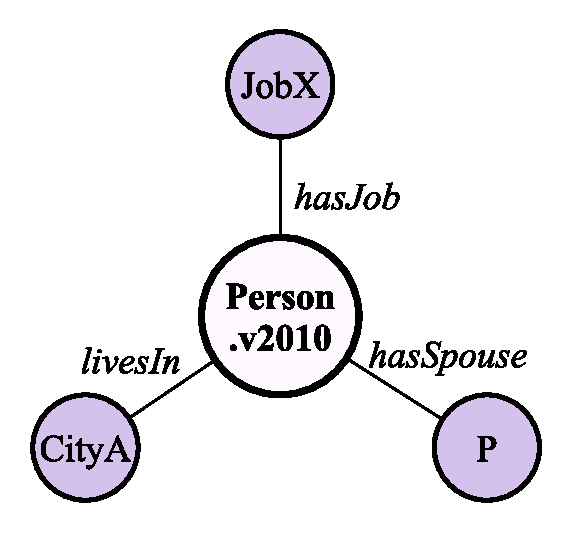
\includegraphics[width=\textwidth]{images/2010.pdf}
            \caption{2010}
            \label{fig:v2010}
        \end{subfigure}
        & 
        \begin{subfigure}[t]{0.19\textwidth}
            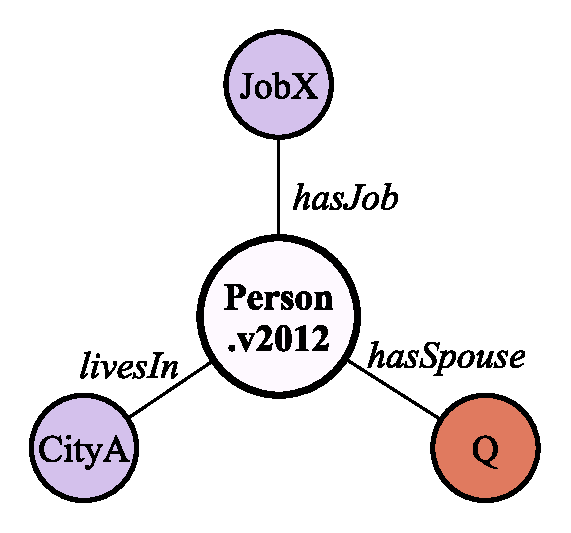
\includegraphics[width=\textwidth]{images/2012.pdf}
            \caption{2012}
            \label{fig:v2012}
        \end{subfigure} 
        \\
        \begin{subfigure}[t]{0.19\textwidth}
            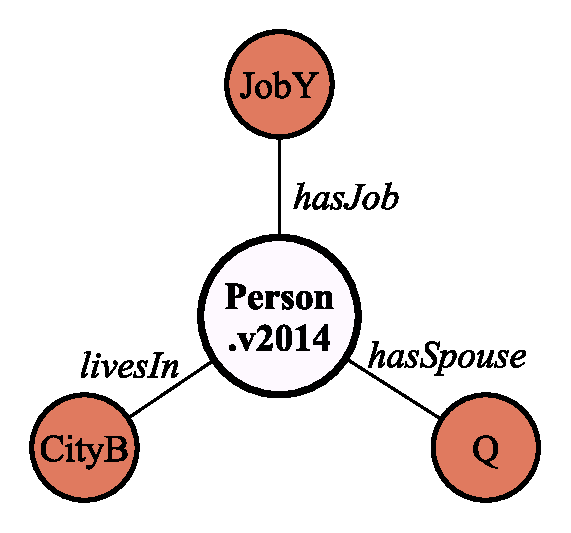
\includegraphics[width=\textwidth]{images/2014.pdf}
            \caption{2014}
            \label{fig:v2014}
        \end{subfigure} 
        & 
        \begin{subfigure}[t]{0.19\textwidth}
            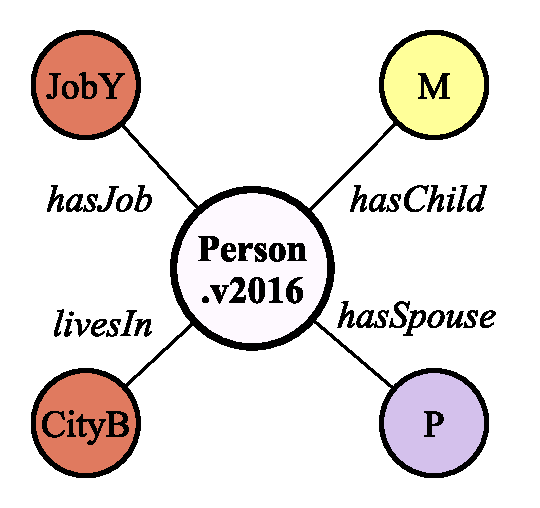
\includegraphics[width=\textwidth]{images/2016.pdf}
            \caption{2016}
            \label{fig:v2016}
        \end{subfigure}
    \end{tabular}
    &
    \begin{subfigure}[t]{0.40\textwidth}
        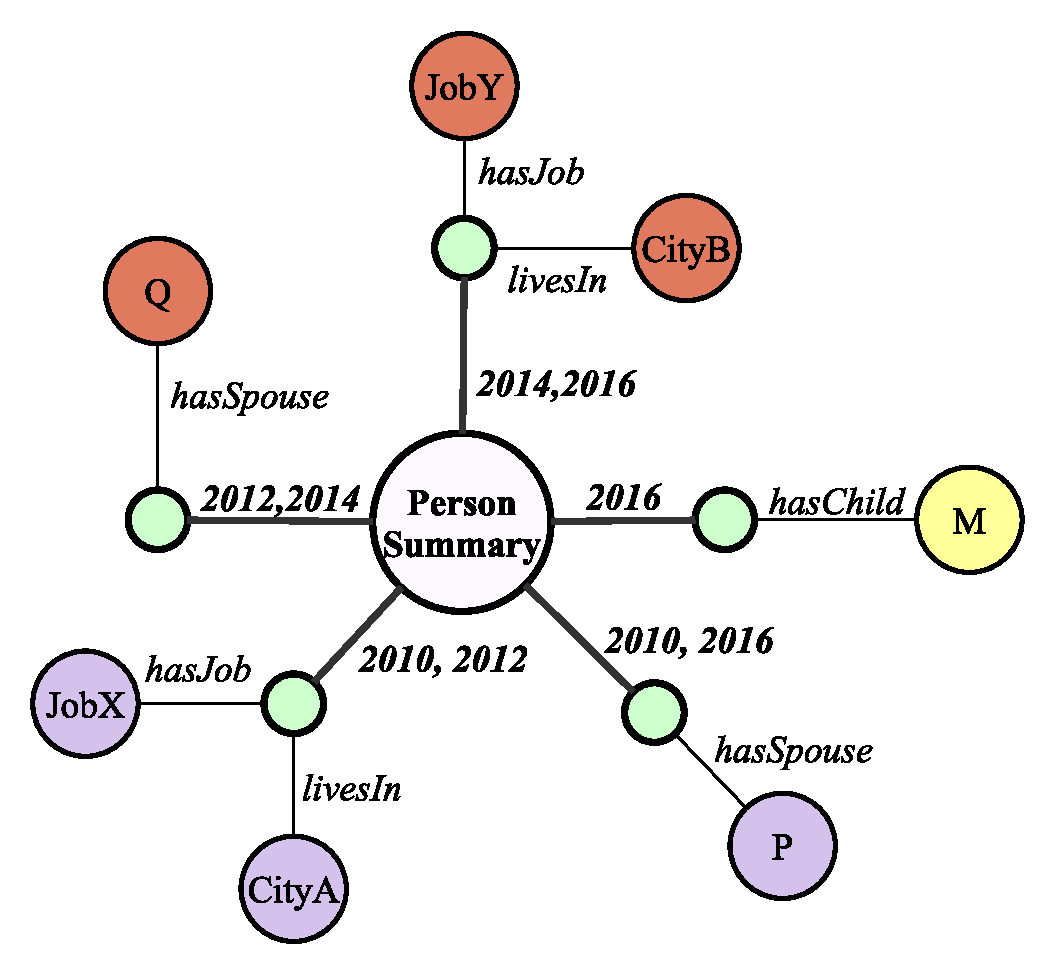
\includegraphics[width=\textwidth]{images/summary.pdf}
        \caption{Summary Representation}
        \label{fig:summary}
    \end{subfigure}
\end{tabular}
\caption{Visual representation of a person info obtained from four yearly molecules.}
\label{fig:motivation}
\end{figure*}

\section{Related Work}
\label{sec:related}
Knowledge graphs are becoming increasingly dynamic in nature and approaches have been proposed~\cite{Umbrich2010} to (i) detect changes during their evolution, (ii) represent change information (using vocabularies) and (iii) propagate changes to replicas or federated systems~\cite{Endris2015}. 
Approaches for change detection mainly focus on computing ``deltas'' (or changesets\footnote{\url{https://www.w3.org/2009/12/rdf-ws/papers/ws07} (accessed on 22/02/2019)}) between two versions of a knowledge graph at different granularity levels~\cite{Umbrich2010}: dataset, resource and statement level. 
The Talis Changeset Vocabulary\footnote{\url{http://vocab.org/changeset/schema} (accessed on 22/02/2019)} defines a set of terms for describing changes to resource descriptions. In the context of this vocabulary, a resource description is the set of triples that includes a description of a resource.
The DELTA-LD framework detects and classifies the changes between two versions of a linked dataset and represents them with the DELTA-LD change model~\cite{Singh2018}. 
DSNotify~\cite{Popitsch2011} is a change-detection system capable of detecting and fixing broken links between resources in two different versions of a dataset.
In~\cite{Roussakis2015}, in order to study the dynamics of LOD, the authors propose a framework for detecting and analysing changes and the evolution history of LOD datasets. Moreover, changes are automatically categorised according to their level of complexity and are represented using an ontology, hence allowing SPARQL to be used to query data changes. Specific queries need to be constructed in order to extract information about the history of changes for a particular class/entity across different versions. In contrast, our approach allows for automatic extraction and exploration of all changes of a class/entity over time.

Producing a summary of an entity evolution can be also tackled as an integration problem. 
Integration frameworks can be used to solve the problem of extracting the temporal evolution of an entity.
In this regard, a central part of this work is represented by the MINTE approach \cite{CollaranaGRV0A17}. We adopt the fusion policies for data integration described by Collarana et al. in order to produce a temporal evolution summary of entities across different versions of a knowledge graph.
Similar to MINTE, ODCleanStore~\cite{MichelfeitK12} is an ETL framework for integrating RDF data. It relies on SILK to perform instance matching and provides custom data fusion modules to merge the data of the discovered matches.
%Other efforts to produce a unified view from RDF graphs are often combined with federated SPARQL query engines, e.g., ANAPSID~\cite{AcostaVLCR11}, FedX~\cite{SchwarteHHSS11}, MULDER~\cite{DBLP:conf/dexa/EndrisGLMVA17}.
%Albeit effective in query planning, such engines process raw tuples coming from endpoints and therefore employ only basic integration according to their join operators.  
%Requiring many and complex queries to be written.
The aim of the said integration frameworks is to map different data sources with possibly varying schema, i.e., they perform inter-schema mapping. However, even in these cases, creating a summarized view of an entity could only be supported on a superficial level by processing and filtering query results.
Hence, we identify the need for an approach to automatically produce summaries of entities' evolution, as described in the following sections.

\section{The Approach}
\label{sec:comet}

\begin{figure*}[t]
    \centering
    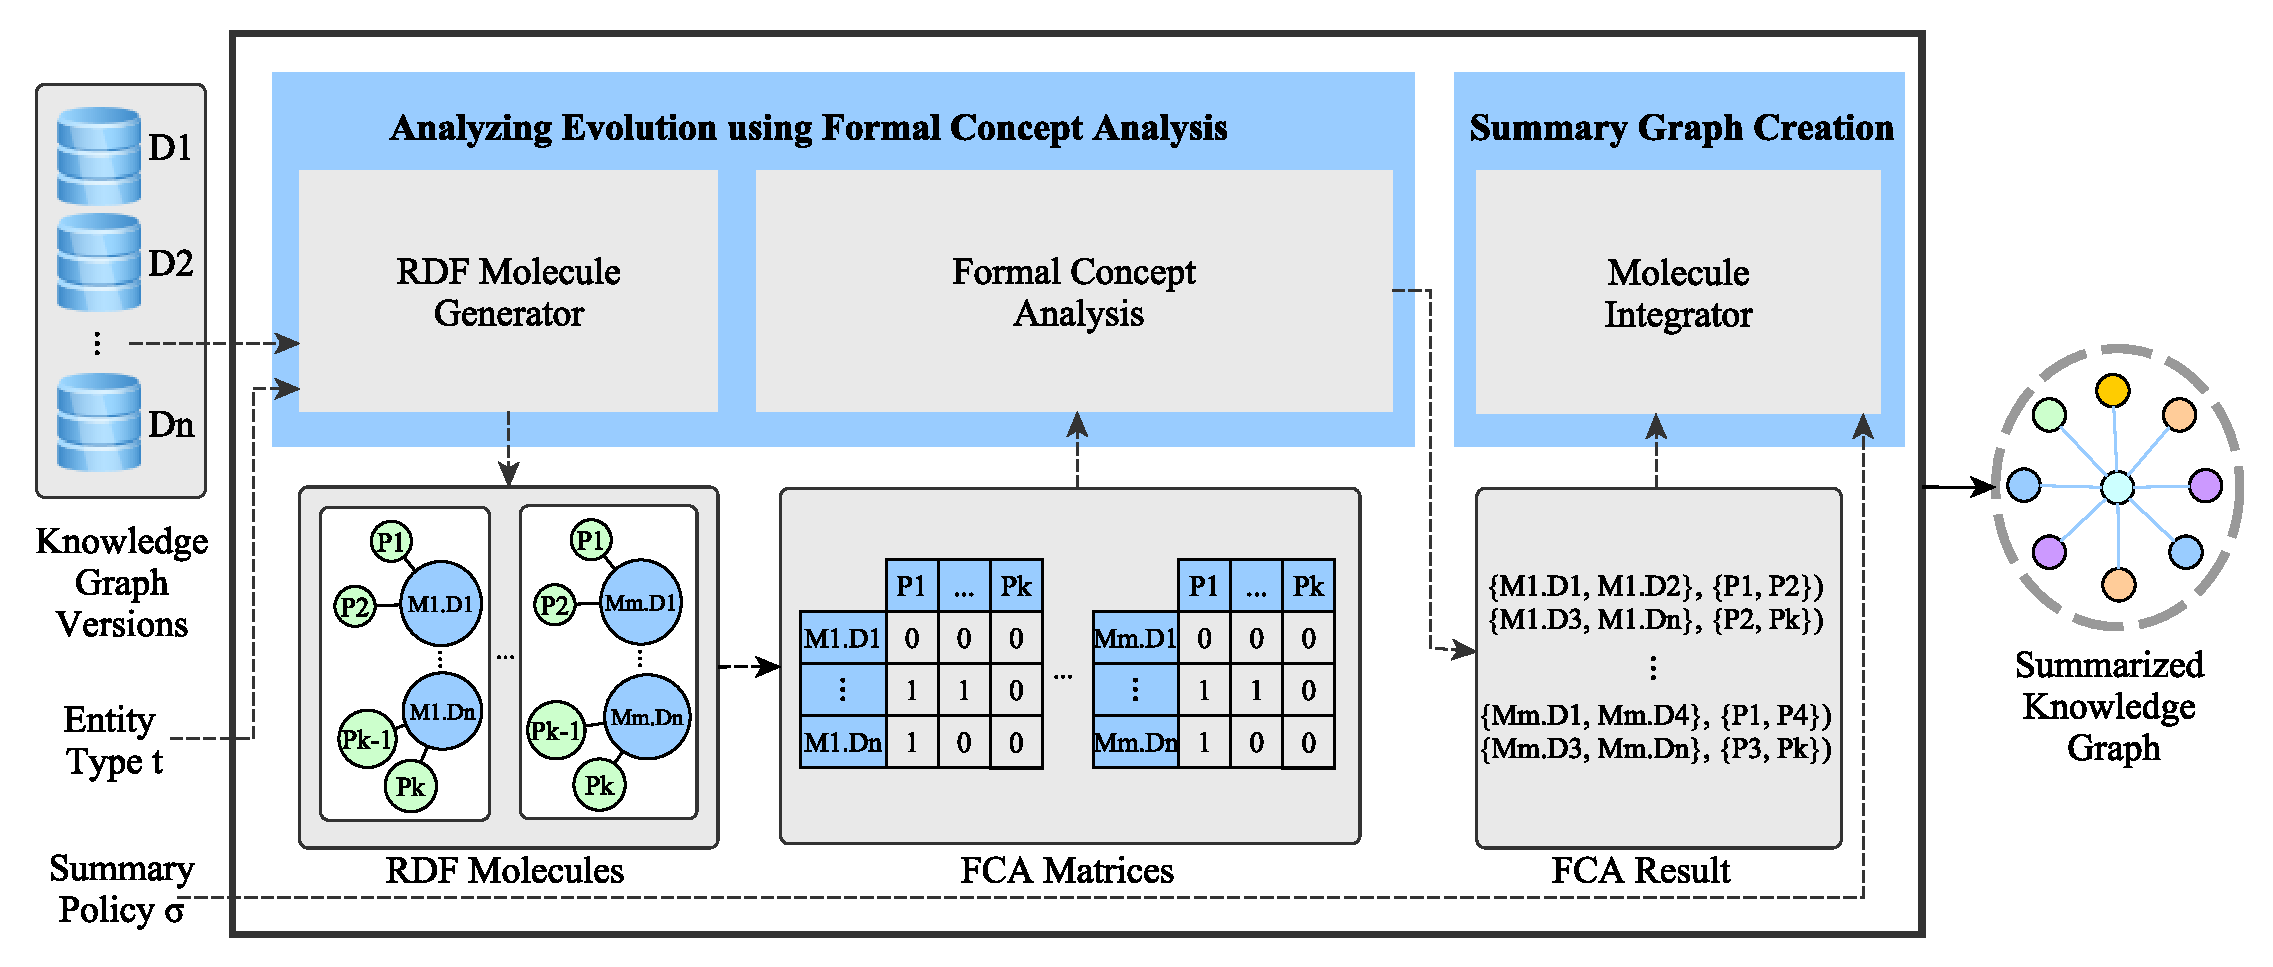
\includegraphics[width=0.9\linewidth]{images/architecture.pdf}
    \caption{The approach receives a set of knowledge graph versions, an entity type, and a summary policy. 
    The output is the entity summaries describing the evolution of knowledge among the different versions of the knowledge graph.}
    \label{fig:architecture}
\end{figure*}

\subsection{Preliminaries}
Given different versions of a knowledge graph, e.g., DBpedia 2010, 2012, 2014, and 2016, and an entity type, e.g., Person.
Our approach automatically produces a summary of evolution over time of the entities under the specified type.
Each entity summary is composed of the evolution of properties and relations among these entities.
To better understand our approach, we define the main concepts, i.e., RDF Molecule, Formal Concept Analysis and Fusion Policies, respectively.

\begin{definition}[RDF Molecule~\cite{fernandez2014efficient}]
\label{def:molecule}
If G is a given RDF Graph, we define an RDF Molecule $M$ as a sub-graph of G such that,
\begin{equation*}
M = \{t_1,\dots, t_n\}, \forall (i,j) \in \{1,\dots,n\}^2 \left( subject(t_i) = subject(t_j) \right)
\end{equation*} where \textit{\(t_1,\dots,t_n\)} denote the triples in $M$. 
In other words, an RDF Molecule $M$ consists of triples which have the same subject.
The RDF molecules are used as unit to produce the entity summary.
\end{definition}

\begin{definition}[Formal Concept Analysis~\cite{vychodil2008new}] aims at describing the relationships between objects and their attributes by considering binary data tables.
In our approach, we apply the algorithm proposed by V. Vychodil~\cite{vychodil2008new}, transforming RDF molecules into the binary data table it requires.
Formal concepts are defined as conceptual clusters found within entity-property data tables.
These data tables have rows corresponding to entities, and columns corresponding to the properties of those entities.
Formal concepts are a set of $<A,B>$ pairs where $A$ is the set of entities, $B$ is a set of properties, and all the entities in $A$ contain all the properties in $B$.
$A$ is known as \emph{extent} and $B$ is known as \emph{intent}.
\label{def:fca}
\end{definition}

\begin{definition}[Fusion Policy~\cite{CollaranaGRV0A17}]
To produce a temporal evolution summary of entities spread over different versions of a knowledge graph, we resort to the concept of fusion policies defined by Collarana et al.~\cite{CollaranaGRV0A17}. 
A fusion policy is a set of rules operating on the triple level, which are triggered by a certain combination of predicates and objects. 
%Fusion policies resemble flexible filters tailored for specific tasks, e.g., keep all literals with different language tags or discard all except one, replace one predicate with another, or simply merge all predicate-value pairs of given molecules. 
Fusion policies resort to an ontology $O$ to resolve possible conflicts and inequalities on the levels of resources, predicates, objects and literals.
\label{def:fpolicy}
\end{definition}

In this paper, we employ RDF molecules, Formal Concept Analysis and Fusion Policies to address the following problem: given a set of versions of RDF knowledge graphs, build an evolution summary of specific entities.
The following section introduces and describes the architecture of our approach.

%\begin{definition}[Formal concept analysis]
%Formal concepts are computed in \cite{vychodil2008new} by using the two procedures outlined in: generate(B,\textit{y}) and closure(B,\textit{y}). 
%The procedure generate(B,\textit{y}) is recursively generates all the intents that are possible in an input object-attribute table using a depth-first search. 
%closure(B,\textit{y}) is a helper procedure that checks whether or not a computed intent is valid or not by computing its closure.
%Intents are characterized by their closure properties, so this procedure helps in identifying if a generated intent D belongs to the formal concept $<A,B>$.
%\end{definition}

\subsection{Architecture}
Grounded on the semantic integration technique proposed by Collarana et al.~\cite{CollaranaGRV0A17}, we propose a pipeline able to automatically create summaries of RDF entity evolution. 
Thus, a solution to \textit{summarizing entity temporal evolution} out of different versions of an RDF knowledge graph is provided.

We propose a three-fold approach in order to identify equivalent entities in different versions of a knowledge graph and summarizing the evolution of those entities, thus providing a solution to the problem of \emph{summarizing entity temporal evolution} in RDF knowledge graphs. 
This approach has three essential components. 
First, the pipeline takes input a set of knowledge graphs representing different temporal versions of the same knowledge graph. These graphs are then converted into a set of RDF molecules, from which molecules that represent the same real-world entity are grouped together. 
Each group of equivalent molecules are then converted into an $M \times N$ binary matrix.
Second, the $M \times N$ matrix is supplied to the FCA component which performs formal concept analysis to summarize the temporal evolution of the molecules. 
Third, a summary fusion policy is applied to each output of the FCA component in order to produce a set of summary molecules. Each summary molecule represents the temporal evolution of a single entity over the knowledge graph versions taken as input.
Figure~\ref{fig:architecture} depicts the main components of this architecture.

\subsection{Conversion of Knowledge Graphs to Groups of Equivalent RDF Molecules}
\label{sec:step1}
The pipeline receives any number of Knowledge Graphs $\phi_1(D)$, $\phi_2(D)$,\ldots,$\phi_n(D)$ as input where $1, 2, \ldots n$ represent the different temporal versions of the same Knowledge Graph $\phi(D)$.
First each graph is individually converted into sets of RDF molecules.
As defined in Preliminaries (see \S\ref{def:molecule}), RDF molecules consist of triples that have the same subject.
Thus we obtain RDF molecule sets $S_1, S_2 \ldots S_n$ which correspond to graphs $\phi_1(D), \phi_2(D) \ldots  \phi_n(D)$ respectively.
The pipeline then identifies equivalent molecules within $S_1, S_2 \ldots S_n$.
As $\phi_1(D), \phi_2(D) \ldots  \phi_n(D)$ are different temporal versions of the same knowledge graph, it can be inferred that there exists equivalent molecules $M_1, M_2 \ldots M_n$ such that $M_1 \in S_1, M_2 \in S_2 \ldots M_n \in S_n$ and $M_1, M_2 \ldots M_n$ all represent the same real-world entity.
For the sake of simplicity it is assumed here that equivalent entities retain the same URI. 
Practically, semantic similarity measures as demonstrated in \cite{CollaranaGRV0A17} can also be integrated with this pipeline to identify equivalent entities in cases where the URI is different.

The equivalent RDF Molecules are then grouped together and each group is converted into a $M \times N$ matrix, where $M$ corresponds to the number of molecules in the group and $N$ corresponds to the number of distinct object or data property the molecules all contain. 
Each element in the matrix $e_{(i, j \rightarrow k)}$ represents whether molecule $M_i$ contains a predicate $j$ that has an object $k$. 
This value can be either \texttt{true} or \texttt{false} and is represented by a 1 and 0, respectively.

Figure~\ref{fig:motivation} presents a scenario where \texttt{Person.v2010, Person.v2012, Person.v2014} and \texttt{Person.v2016} all represent the same real world entity \texttt{Person} from Knowledge Graphs from year 2010, 2012, 2014 and 2016 respectively. 
In this first step of the pipeline, these molecules would be extracted from their respective knowledge graphs, identified as equivalent molecules, and then grouped together.  
This group of molecules would then be converted into a $4 \times 7$ matrix, 4 being the number of molecules in the group and 7 being the total number of distinct object/data properties in all the molecules.
This matrix is shown in Table \ref{tab:matrix}. 
The column headers, i.e. properties for this matrix are shown separately in Table \ref{tab:props}.
Once the $M \times N$ matrix has been created, it is then passed on to the next component in the pipeline to perform Formal Concept Analysis and summarize the temporal evolution in equivalent RDF entities.

\begin{table*}[t]
\begin{subtable}[b]{.35\linewidth}
\centering
{
    \begin{tabular}{llllllll} 
    \toprule
    & P1 & P2 & P3 & P4 & P5 & P6 & P7\\ \midrule
    M1 & 1 & 0 & 1 & 0 & 1 & 0 & 0\\ 
    M2 & 1 & 0 & 1 & 0 & 0 & 1 & 0\\ 
    M3  & 0 & 1 & 0 & 1 & 0 & 1 & 0\\
    M4  & 0 & 1 & 0 & 1 & 1 & 0 & 1\\ \bottomrule
    \end{tabular}}
\caption{FCA Input}\label{tab:matrix}
\end{subtable}%
\begin{subtable}[b]{.24\linewidth}\centering
{
 \begin{tabular}{lr}
    \toprule
    Molecule & Property \\ \midrule
    M1 & P1,P3,P5  \\ 
    M2 & P1,P3,P6  \\ 
    M3 & P2,P4,P6  \\ 
    M4 & P2,P4,P5,P7 \\ 
    M1, M2 & P1,P3 \\ 
    M2, M3 & P6 \\ 
    M3, M4 & P2,P4 \\ 
    M1, M4 & P5 \\ \bottomrule
 \end{tabular}
}
\caption{FCA Output}\label{tab:result}
\end{subtable}
\begin{subtable}[b]{.15\linewidth}\centering
{
 \begin{tabular}{lr}
    \toprule
    \multicolumn{1}{c}{}& Molecule \\ \midrule
    M1 & Person.v2010  \\ 
    M2 & Person.v2012  \\ 
    M3 & Person.v2014  \\
    M4 & Person.v2016 \\ \bottomrule
 \end{tabular}
}
\caption{Molecules}\label{tab:props}
\end{subtable}
\begin{subtable}[b]{.25\linewidth}\centering
{
 \begin{tabular}{lr}
    \toprule
    \multicolumn{1}{c}{}& Property \\ \midrule
    P1 & \texttt{livesIn} $\rightarrow$ \emph{CityA}  \\ 
    P2 & \makecell{\texttt{livesIn} $\rightarrow$ \emph{CityB}}  \\ 
    P3 & \makecell{\texttt{hasJob} $\rightarrow$ \emph{JobX}}  \\ 
    P4 & \makecell{\texttt{hasJob} $\rightarrow$ \emph{JobY}} \\ 
    P5 & \makecell{\texttt{isSpouseOf} $\rightarrow$ \emph{P}    } \\ 
    P6 & \makecell{\texttt{isSpouseOf} $\rightarrow$ \emph{Q}    } \\ 
    P7 & \makecell{\texttt{isFatherOf} $\rightarrow$ \emph{M}    } \\ \bottomrule
 \end{tabular}
}
\caption{Properties}\label{tab:props}
\end{subtable}
\caption{Preparing equivalent RDF Molecules for Formal Concept Analysis: \texttt{Person} molecules from 4 different knowledge graph versions are grouped and compiled into a matrix for performing formal concept analysis. Rows correspond to each molecule, while columns correspond to distinct properties.}\label{tab:fca}
\end{table*}

\begin{figure}[t]
    \centering
    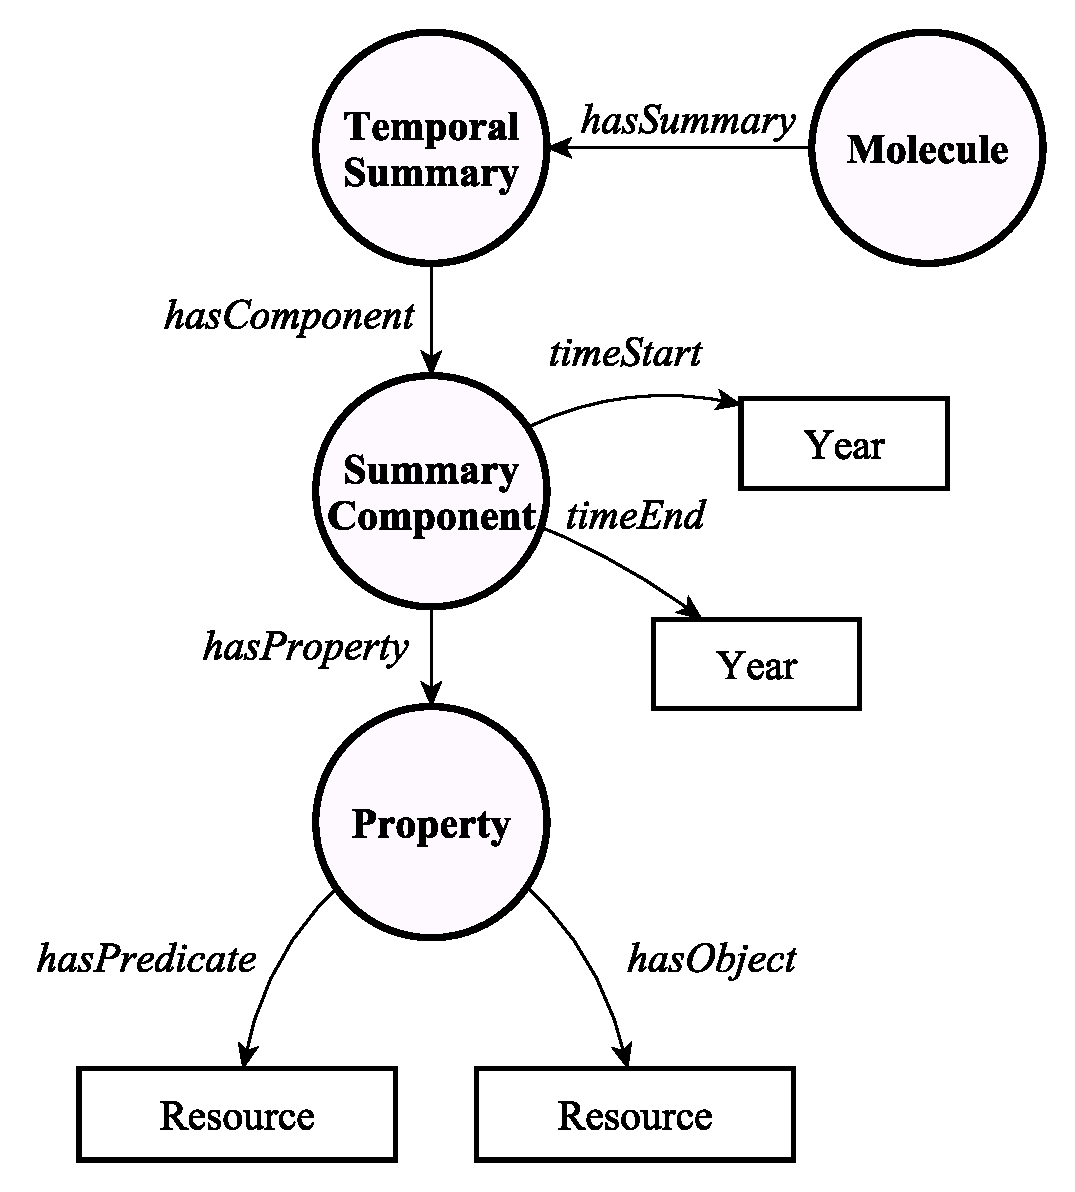
\includegraphics[width=0.6\linewidth]{images/ontology.pdf}
    \caption{The ontology used to apply summary fusion policy for the creation of summary molecules.}
    \label{fig:ontology}
\end{figure}

\subsection{Applying Formal Concept Analysis to Obtain a Summary of Evolution}
\label{sec:step2}
As first mentioned in Definition \ref{def:fca}, formal concept analysis studies binary object-attribute tables to describe the relationship between \emph{objects} and their \emph{attributes}.
Our approach first converts knowledge graphs to RDF molecules.
Within a single knowledge graph, an RDF molecule can be considered as an \emph{object} while its object or data properties can be considered as \emph{attributes}.
When RDF molecules are modeled in this way, we are able to apply the formal concept analysis algorithm to compute formal concepts.
The creation of these binary matrices is discussed in the previous section.

We apply the algorithm by V. Vychodil~\cite{vychodil2008new} on each group of RDF molecules obtained from the previous step.
The algorithm returns a set of formal concepts $<M,P>$ where $M$ is a set of all the molecules that have all the properties contained in $P$. 
In our approach the output $<M,P>$ from formal concept analysis gives us a set of molecules that have the same properties throughout different knowledge graph versions.

Table \ref{tab:fca} demonstrates the input and output of formal concept analysis when applied to the RDF molecules in our motivation example. Table \ref{tab:matrix} shows the $4 \times 7$ binary matrix representing the object-attribute table. Table \ref{tab:result} shows the output of the FCA algorithm when supplied with this matrix. 
It supplies the information of which properties of the molecule has remained the same over which years. 
For example, Table \ref{tab:result} shows us that the entity Person had the same job ({\texttt{hasJob} $\rightarrow$ \emph{JobX}}) and lived in the same city (\texttt{livesIn} $\rightarrow$ \emph{CityA}) over the years 2010 and 2012. 

The output of the FCA algorithm is supplied to the next step in order to create summary molecules.

\begin{figure}[t]
    \centering
    {\fontsize{8}{12}\selectfont
    \noindent
    \begin{minipage}[t]{.40\textwidth}
        \vspace{0pt}
        \begin{algorithm}[H]
            \SetNoFillComment
            \SetKwData{Left}{left}\SetKwData{This}{this}\SetKwData{Up}{up}
            \SetKwFunction{Union}{Union}\SetKwFunction{FindCompress}{FindCompress}
            
            summary $\leftarrow$ list() \tcp*{Initialize empty list}
            n $\leftarrow$ FCAResult.length\;
            \For{$j \leftarrow$1 \KwTo n}{
                $(M,P) \leftarrow$ FCAResult$[j]$\;
                \If{$M.length \geq 1$ and $P.length \geq 0$}{
                    summary $\leftarrow$ summary $+$ $(M,P)$ \;
                    FCAResult $\leftarrow$ FCAResult $-$ $(M,P)$ \;
                }
            }
            n $\leftarrow$ FCAResult.length \tcp*{Recompute length}
            m $\leftarrow$ summary.length\;
            \For{$j \leftarrow$1 \KwTo n}{
                $(M,P) \leftarrow$ FCAResult$[j]$\;
                \If{$M.length \eq 1$ and $P.length \geq 0$}{
                    \For{$k \leftarrow$1 \KwTo m}{
                        $(X,Y) \leftarrow$ summary$[k]$\;
                        \If{$M[1] \in X$}{
                            $P$ $\leftarrow$ $P$ $-$ $Y$    
                        }
                    }
                    \If{$P.length \geq 0$}{
                    summary $\leftarrow$ summary $+$ $(M,P)$ \;
                    }
                }
            }
            \Return{summary}
            \caption{CreateSummary(FCAResult)}
        \end{algorithm}
    \end{minipage}
    }
    \caption{Algorithm for selecting distinct properties that form the \emph{Summary Molecule}}
    \label{algos}
\end{figure}

\subsection{Applying Fusion Policy to Integrate Summary into Knowledge Graph}
\label{sec:step3}
To integrate the result obtained from the formal concept analysis algorithm, we resort to extend the fusion policies defined by Collarana et al.~\cite{CollaranaGRV0A17}. 
They defined the following:  
(1) the \emph{Union Policy}, which includes all predicates-object pairs, removing the one that are syntactically the same;
(2) the \emph{Subproperty Policy}, which tracks if a property of one RDF molecule is an \texttt{rdfs:subPropertyOf} of a property of another RDF molecule, i.e.,  
$\{r_1, p_1, A\}, \{r_2, p_1, B\} + O + subPropertyOf(p_1,$ $ p_2) \models \{\sigma_r(r_1,r_2), p_2, \sigma_{v}(A,B)\}$.
As a result of applying this policy,  the property $p_1$ is replaced with a more general property $p_2$;
and (3) the \emph{Authority Graph Policy}, which allows for defining one RDF graph as a prevalent source selecting its properties in case of property conflicts, i.e., properties annotated as \texttt{owl:FunctionalProperty}, equivalent properties \texttt{owl:equivalent\-Property}, and equivalent classes annotated with \texttt{owl:equivalent\-Class} or \texttt{owl:sameAs}.

For the purpose of creating a \emph{compact summary} of the temporal evolution of RDF molecules, we define an additional fusion policy called the \emph{Summary Policy}. \emph{Summary Policy} selects distinct properties from the output of the FCA algorithm, and follows the ontology shown in Figure \ref{fig:ontology} to create a \emph{temporal summary graph}.
A visual representation of the temporal summary graph according to our motivation example is shown in Figure \ref{fig:summary}.
For the sake of compactness, the summary graph is designed to have only one occurrence of each distinct property. 

A \emph{temporal summary graph} is created by first selecting all distinct properties out of the result obtained from the previous step. 
This is done by applying the algorithm shown in Figure \ref{algos} on a list of results like the one shown in Table \ref{tab:result}.
The algorithm takes as input the result $R$ of the FCA algorithm.
For every $(M,P) \in R, |M| = 1$,
it returns $(M,P')$ such that, 
$\forall (X,Y) \in R$ 
where $|X|>1$ and $M\in X$, $P' = P \cap Y$ and $P' \neq \phi$.

For example, for the row [\{M4\}, \{P2,P4,P5,P7\}] in Table \ref{tab:result}, the above algorithm is applied to obtain [\{M4\}, \{P7\}], i.e. [\{Person.v2016\}, \{\texttt{hasChild} $\rightarrow$ \emph{M}\}].
This can be seen in Figure~\ref{fig:summary}, where the property \texttt{hasChild} $\rightarrow$ \emph{M} occurs only under the summary component of 2016. 
Every other property in Person.v2016 occurs also in other versions of the Person entity. 
This is represented in the summary graph under the summary components of (2010,2016) and (2014, 2016). 
The summary graph allows the possibility to reconstruct the original versions of the molecules.
For example, in order to obtain the 2010 version of the Person molecule, it is only needed to select the edges of the summary graph that are annotated with the year 2010, and apply \emph{Union Policy}.

\balance

\section{Conclusions and Future work}
In this paper, we envision an approach for creating entity summaries automatically out of different temporal versions of a knowledge graph.
To do so, the proposed approach utilizes the concepts of RDF molecules, Formal Concept Analysis, and Fusion Policies.
We have explained the architecture and pipeline where only one parameter is needed, i.e., the entity type.
%Although the elements in this version of the paper are quite simple, e.g, the ontology, they can be extended and further develop to empower the approach.
The entity evolution summaries created by the approach may serve to create documentation, to display a visualization of the entity evolution, or to make an analysis of changes.
As future work, we plan to implement and evaluate the approach considering its scalability and applicability.

%\noindent
\textbf{Acknowledgements:}
%\subsubsection{Acknowledgements:}
This work is supported by the German Ministry of Education and Research (BMBF) in the context of the project MLwin (\quotes{Maschinelles Lernen mit Wissensgraphen}, grant no. 01IS18050F).

%
% ---- Bibliography ----
%
\bibliographystyle{abbrv}
\bibliography{bibliography.bib}

\end{document}



% \begin{figure}[t]
%     \centering
%     {\fontsize{8}{12}\selectfont
%     \noindent
%     \begin{minipage}[t]{.47\textwidth}
%         \vspace{0pt}
%         \begin{algorithm}%[H]
%             \SetKwData{Left}{left}\SetKwData{This}{this}\SetKwData{Up}{up}
%             \SetKwFunction{Union}{Union}\SetKwFunction{FindCompress}{FindCompress}
%             \For{$j\leftarrow 0$ \KwTo $n$}{
%                 $D[j]\leftarrow 1$\;
%             }
%             \ForEach{$i$ in $rows[y]$}{
%                 $match\leftarrow \textrm{True}$\;
%                 \For{$j\leftarrow 0$ \KwTo n}{
%                     %\If{$B[j]=1$ \& $context[i,j]=0$}{
%                     \If{$\left\{\begin{array}{l}B[j]=1\\context[i,j]=0\end{array}\right.$}{
%                         $match\leftarrow\mathrm{False}$\;
%                         \textbf{break for loop}\;
%                     }
%                 }
%                 \If{$match = \textrm{True}$}{
%                     \For{$j\leftarrow 0$ \KwTo n}{
%                         \If{$context[i,j]=0$}{
%                             $D[j]\leftarrow 0$\;
%                         }
%                     }
%                 }
%             }
%             \Return{$D$}
%             \caption{closure(B,$y$)}
%         \end{algorithm}
%     \end{minipage}
%     ~
%     \begin{minipage}[t]{.47\textwidth}
%         \vspace{0pt}
%         \begin{algorithm}%[H]
%             \SetNoFillComment
%             \SetKwData{Left}{left}\SetKwData{This}{this}\SetKwData{Up}{up}
%             \SetKwFunction{Union}{Union}\SetKwFunction{FindCompress}{FindCompress}
            
%             process $B$ \tcp*{Printing $B$}
%             \If{$B=Y~|~y>n$}{
%                 \Return{}
%             }
%             \For{$j\leftarrow y$ \KwTo n}{
%                 \If{$B[j]=0$}{
%                     $B[j]\leftarrow1$\;
%                     $D\leftarrow\textrm{closure(B,j)}$\;
%                     $skip\leftarrow\textrm{False}$\;
%                     \For{$k\leftarrow0$ \KwTo $j-1$}{
%                         \If{$D[k]\neq B[k]$}{
%                             $skip\leftarrow\textrm{True}$\;
%                             \textbf{break for loop}\;
%                         }
%                     }
%                     \If{$skip=\textrm{False}$}{
%                         \textrm{generate($D$,$j+1$)}\;
%                     }
%                     $B[j]\leftarrow 0$\;
%                 }
%             }
%             \Return{}
%             \caption{generate(B,$y$)}
%         \end{algorithm}
%     \end{minipage}
%     }
%     \caption{Implemented algorithms (extended from~\cite{vychodil2008new}).}
%     \label{algos}
% \end{figure}





\captionsetup[subfigure]{labelformat=empty}
\begin{figure*}[t]
\centering
\begin{tabular}{cccc}
        \begin{subfigure}[t]{0.19\textwidth}
        \includegraphics[width=\textwidth]{images/v2010.png}
        \caption{(a) 2010}
        \label{fig:v2010}
    \end{subfigure}
    & 
    \begin{subfigure}[t]{0.19\textwidth}
        \includegraphics[width=\textwidth]{images/v2012.png}
        \caption{(b) 2012}
        \label{fig:v2012}
    \end{subfigure} 
    & 
    \multicolumn{2}{c}{\multirow{2}{*}[\dimexpr1.15in-\baselineskip-0.5\abovecaptionskip-0.8ex\relax]{
        \begin{subfigure}[t]{0.40\textwidth}
            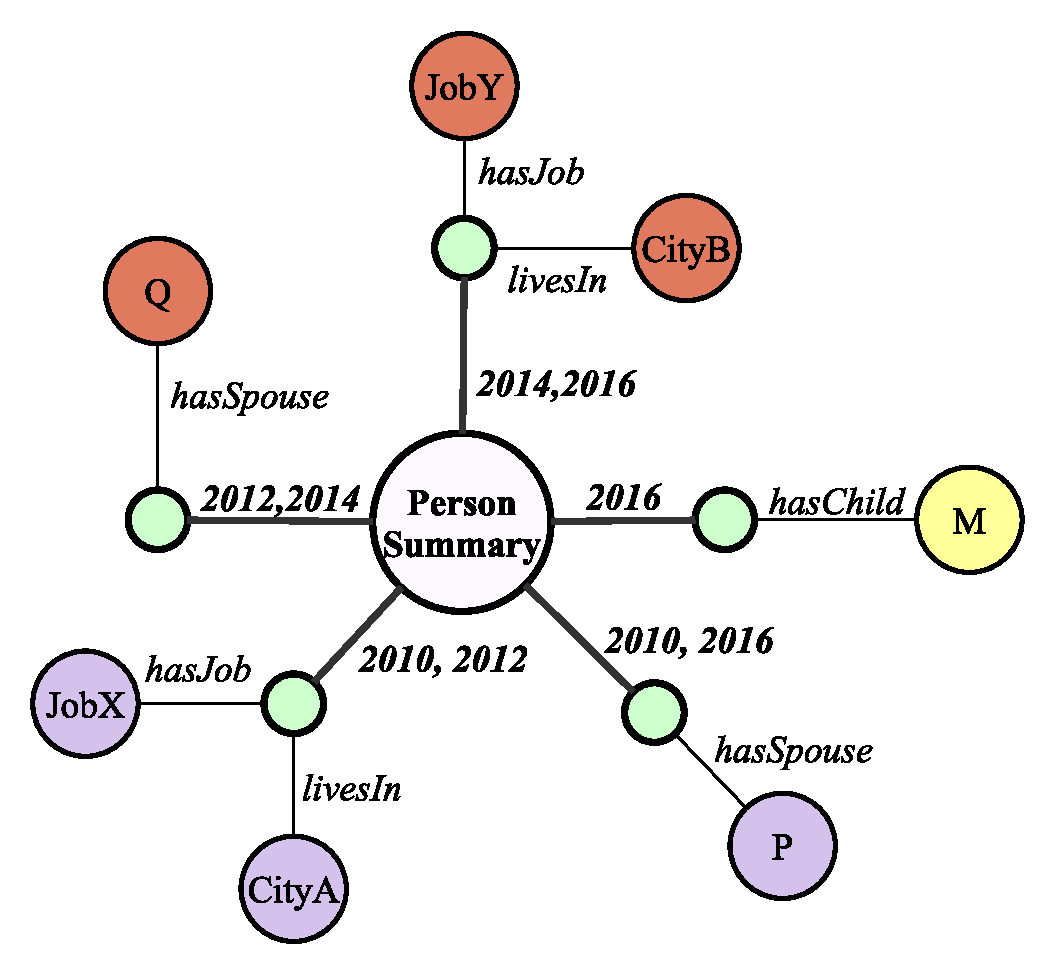
\includegraphics[width=\textwidth]{images/summary.png}
            \caption{(c) Summary Representation}
            \label{fig:summary}
        \end{subfigure}
    }} 
    \\
    \begin{subfigure}[t]{0.19\textwidth}
        \includegraphics[width=\textwidth]{images/v2014.png}
        \caption{(d) 2014}
        \label{fig:v2014}
    \end{subfigure} 
    & 
    \begin{subfigure}[t]{0.19\textwidth}
        \includegraphics[width=\textwidth]{images/v2016.png}
        \caption{(e) 2016}
        \label{fig:v2016}
    \end{subfigure}
\end{tabular}
\caption{Visual representation of a person info obtained from four yearly molecules.}
\label{fig:motivation}
\end{figure*}

